%
% Modified by Megan Patnott
% Last Change: Jan 18, 2013
%
%%%%%%%%%%%%%%%%%%%%%%%%%%%%%%%%%%%%%%%%%%%%%%%%%%%%%%%%%%%%%%%%%%%%%%%%
%
% Modified by Sameer Vijay
% Last Change: Wed Jul 27 2005 13:00 CEST
%
%%%%%%%%%%%%%%%%%%%%%%%%%%%%%%%%%%%%%%%%%%%%%%%%%%%%%%%%%%%%%%%%%%%%%%%%
%
% Sample Notre Dame Thesis/Dissertation
% Using Donald Peterson's ndthesis classfile
%
% Written by Jeff Squyres and Don Peterson
%
% Provided by the Information Technology Committee of
%   the Graduate Student Union
%   http://www.gsu.nd.edu/
%
% Nothing in this document is serious except the format.  :-)
%
% If you have any suggestions, comments, questions, please send e-mail
% to: ndthesis@gsu.nd.edu
%
%%%%%%%%%%%%%%%%%%%%%%%%%%%%%%%%%%%%%%%%%%%%%%%%%%%%%%%%%%%%%%%%%%%%%%%%

%
% Chapter 3
%

\chapter{COMPARISONS WITH THE EWALD SUM}
\label{chap:compEwald}

In the previous chapter, I briefly discussed the short-ranged nature of the electrostatic interaction in the crystalline environment. This chapter discusses the property of the electrostatic interactions in more detail and extend the idea of the short-ranged nature of the interaction in the case of liquid simulation. I present the comparison of the energies, forces and torques calculated using real-space methods with the Ewald sum. Additionally I derive different static and dynamic properties using newly developed real-space methods and compare result with the Ewald. Finally I report on the conservation of total energy in the molecular dynamics simulation for the various real-space and Ewald methods.  

\section{Introduction}

As we mentioned earlier Wolf \textit{et al.}\cite{Wolf99} proposed a real space $O(N)$ method for calculating electrostatic interactions between point charges. They argued that the effective Coulomb interaction in most condensed phase systems is effectively short
ranged.\cite{Wolf92,Wolf95} For an ordered lattice (e.g., when
computing the Madelung constant of an ionic solid), the material can
be considered as a set of ions interacting with neutral dipolar or
quadrupolar ``molecules'' giving an effective distance dependence for
the electrostatic interactions of $r^{-5}$ (see Fig.~\ref{fig:schematic1}). If one views the \ce{NaCl} crystal as a simple
cubic (SC) structure with an octupolar \ce{$\mathrm{(NaCl)_4$}} basis, the
electrostatic energy per ion converges more rapidly to the Madelung
energy than the dipolar approximation.\cite{Wolf92} To find the
correct Madelung constant, Lacman suggested that the NaCl structure
could be constructed in a way that the finite crystal terminates with
complete \ce{$\mathrm{(NaCl)_4$}} molecules.\cite{Lacman65} The central ion sees
what is effectively a set of octupoles at large distances. These facts
suggest that the Madelung constants are relatively short ranged for
perfect ionic crystals.\cite{Wolf99} For this reason, careful
application of Wolf's method can provide accurate estimates of
Madelung constants using relatively short cutoff radii.

Direct truncation of interactions at a cutoff radius creates numerical
errors.  Wolf \textit{et al.} suggest that truncation errors are due
to net charge remaining inside the cutoff sphere.\cite{Wolf99} To
neutralize this charge they proposed placing an image charge on the
surface of the cutoff sphere for every real charge inside the cutoff sphere. These charges are present for the evaluation of both the pair
interaction energy and the force, although the force expression
maintains a discontinuity at the cutoff sphere.  In the original Wolf
formulation, the total energy for the charge and image were not equal
to the integral of the force expression, and as a result, the total
energy would not be conserved in molecular dynamics (MD)
simulations.\cite{Zahn02} Zahn \textit{et al.}, and Fennell and
Gezelter later proposed shifted force variants of the Wolf method with
commensurate force and energy expressions that do not exhibit this
problem.\cite{Zahn02,Gezelter06} Related real-space methods
were also proposed by Chen \textit{et al.} \cite{Chen04,Chen06,Denesyuk08,Rodgers06}
and by Wu and Brooks.\cite{Wu05} Recently, Fukuda has successfully
used additional neutralization of higher order moments for systems of
point charges.\cite{Fukuda13}

\begin{figure}
  \centering
  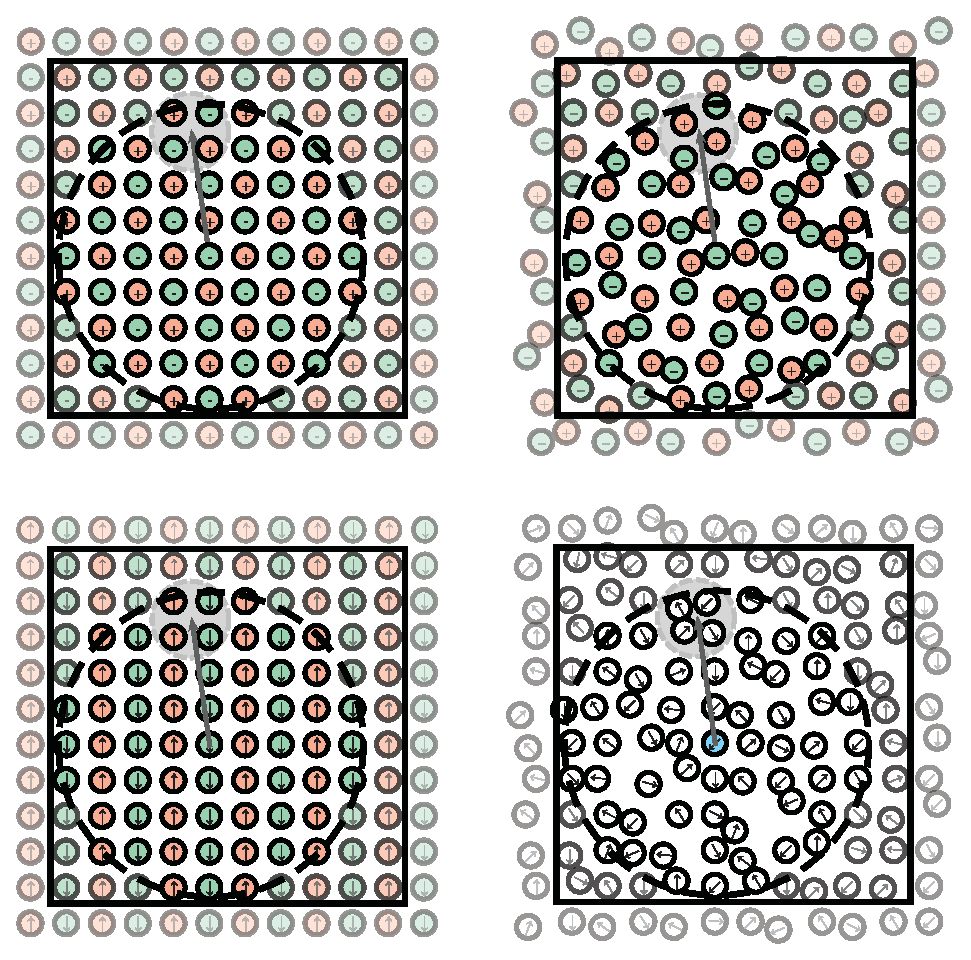
\includegraphics[width=\linewidth]{schematic.eps}
  \caption{Top: Ionic systems exhibit local clustering of dissimilar
    charges (in the smaller grey circle), so interactions are
    effectively charge-multipole at longer distances.  With hard
    cutoffs, motion of individual charges in and out of the cutoff
    sphere can break the effective multipolar ordering.  Bottom:
    dipolar crystals and fluids have a similar effective
    \textit{quadrupolar} ordering (in the smaller grey circles), and
    orientational averaging helps to reduce the effective range of the
    interactions in the fluid.  Placement of reversed image multipoles
    on the surface of the cutoff sphere recovers the effective
    higher-order multipole behavior. \label{fig:schematic1}}
\end{figure}

One can make a similar effective range argument for crystals of point
\textit{multipoles}. The Luttinger and Tisza treatment of energy
constants for dipolar lattices utilizes 24 basis vectors that contain
dipoles at the eight corners of a unit cube.\cite{LT} Only three of
these basis vectors, $X_1, Y_1, \mathrm{~and~} Z_1,$ retain net dipole
moments, while the rest have zero net dipole and retain contributions
only from higher order multipoles.  The lowest-energy crystalline
structures are built out of basis vectors that have only residual
quadrupolar moments (e.g. the $Z_5$ array). In these low energy
structures, the effective interaction between a dipole at the center
of a crystal and a group of eight dipoles farther away is
significantly shorter ranged than the $r^{-3}$ that one would expect
for raw dipole-dipole interactions.  Only in crystals which retain a
bulk dipole moment (e.g. ferroelectrics) does the analogy with the
ionic crystal break down -- ferroelectric dipolar crystals can exist,
while ionic crystals with net charge in each unit cell would be
unstable.

In ionic crystals, real-space truncation can break the effective
multipolar arrangements (see Fig. \ref{fig:schematic1}), causing
significant swings in the electrostatic energy as individual ions move
back and forth across the boundary.  This is why the image charges are
necessary for the Wolf sum to exhibit rapid convergence.  Similarly,
the real-space truncation of point multipole interactions breaks
higher order multipole arrangements, and image multipoles are required
for real-space treatments of electrostatic energies.

The shorter effective range of electrostatic interactions is not
limited to perfect crystals, but can also apply in disordered fluids.
Even at elevated temperatures, there is local charge balance in an
ionic liquid, where each positive ion has surroundings dominated by
negative ions and vice versa.  The reversed-charge images on the
cutoff sphere that are integral to the Wolf and damped shifted force
(DSF) approaches retain the effective multipolar interactions as the
charges traverse the cutoff boundary.

In multipolar fluids (see Fig. \ref{fig:schematic1}) there is
significant orientational averaging that additionally reduces the
effect of long-range multipolar interactions.  The image multipoles
that are introduced in the Taylor shifted force (TSF), gradient
shifted force (GSF), and shifted potential (SP) methods mimic this effect and reduce the effective range of the multipolar interactions as
interacting molecules traverse each other's cutoff boundaries.

Forces and torques acting on atomic sites are fundamental in driving
dynamics in molecular simulations, and the DSF energy kernel provides
consistent energies and forces on charged atoms within the cutoff
sphere. Both the energy and the force go smoothly to zero as an atom
approaches the cutoff radius. The comparisons of the accuracy these
quantities between the DSF kernel and SPME was surprisingly
good.\cite{Gezelter06} As a result, the DSF method has seen
increasing use in molecular systems with relatively uniform charge
densities. \cite{English08,Kannam13,Forrest12,Louden13,McCann13,Shi13,Tokumasu13}

\section{Methodology}
To understand how the real-space multipole methods behave in computer
simulations, it is vital to test against established methods for
computing electrostatic interactions in periodic systems, and to
evaluate the size and sources of any errors that arise from the
real-space cutoffs.  In the chapter 2 of this series, we compared
the dipolar and quadrupolar energy expressions against analytic
expressions for ordered dipolar and quadrupolar
arrays.\cite{Sauer,LT,Nagai60,Nagai63} In this work, we
used the multipolar Ewald sum as a reference method for comparing
energies, forces, and torques for molecular models that mimic
disordered and ordered condensed-phase systems.  The parameters used
in the test cases are given in Table~\ref{tab:pars}. 

\begin{sidewaystable}
  \caption{The parameters used in the systems used to evaluate the new
    real-space methods.  The most comprehensive test was a liquid
    composed of 2000 soft DQ liquid molecules with 48 dissolved ions (24 \ce{Na+} and 24 \ce{Cl-}
    ions).  This test exercises all orders of the multipolar
    interactions developed in the chapter 2.\label{tab:pars}}
\begin{tabularx}{\textwidth}{r|cc|YYccc|Yccc} \hline
             & \multicolumn{2}{c|}{LJ parameters} &
             \multicolumn{5}{c|}{Electrostatic moments} & & & & \\
 Test system & $\sigma$& $\epsilon$ & $C$ & $D$  &
 $Q_{xx}$ & $Q_{yy}$ & $Q_{zz}$ & mass  & $I_{xx}$ & $I_{yy}$ &
 $I_{zz}$ \\ \cline{6-8}\cline{10-12}
 & (\AA) & (kcal/mol) & (e) & (debye) & \multicolumn{3}{c|}{(debye \AA)} & (amu) & \multicolumn{3}{c}{(amu
 \AA\textsuperscript{2})} \\ \hline
    Soft Dipolar fluid & 3.051 & 0.152 &  & 2.35 & & & & 18.0153 & 1.77&0.6145& 1.155 \\
    Soft Dipolar solid & 2.837 & 1.0   &  & 2.35 & & & & $10^4$  & 17.6 &17.6 & 0 \\
Soft Quadrupolar fluid & 3.051 & 0.152 &  &  & -1&-1&-2.5 & 18.0153 & 1.77&0.6145&1.155  \\
Soft Quadrupolar solid & 2.837 & 1.0   &  &  & -1&-1&-2.5 & $10^4$  & 17.6&17.6&0 \\
      Soft DQ liquid  & 3.051 & 0.152 &  & 2.35 & -1.35&0&-0.68 & 18.0153 & 1.77&0.6145&1.155 \\
              \ce{Na+} & 2.579 & 0.118 & +1& & & & & 22.99 & & &\\
              \ce{Cl-} & 4.445 & 0.1   & -1& & & & & 35.4527& & & \\ \hline
\end{tabularx}
\end{sidewaystable}

The systems consist of pure multipolar solids (both dipole and
quadrupole), pure multipolar liquids (both dipole and quadrupole), a
fluid composed of sites containing both dipoles and quadrupoles
simultaneously, and a final test case that includes ions with point
charges in addition to the multipolar fluid.  The solid-phase
parameters were chosen so that the systems can explore some
orientational freedom for the multipolar sites, while maintaining
relatively strict translational order.  The soft DQ liquid model used
here based loosely on the SSDQO water
model,\cite{Chowdhuri06,Te10vn,Te10ys} but is not itself a
particularly accurate water model.  However, the soft DQ model does
test dipole-dipole, dipole-quadrupole, and quadrupole-quadrupole
interactions at roughly the same magnitudes. The last test case, a
soft DQ liquid with dissolved ions, exercises \textit{all} levels of
the multipole-multipole interactions we have derived so far and
represents the most complete test of the new methods.

In the following section, we present results for the total
electrostatic energy, as well as the electrostatic contributions to
the force and torque on each molecule.  These quantities have been
computed using the SP, TSF, and GSF methods, as well as a hard cutoff,
and have been compared with the values obtained from the multipolar
Ewald sum.  In Monte Carlo (MC) simulations, the energy differences
between two configurations is the primary quantity that governs how
the simulation proceeds. These differences are the most important
indicators of the reliability of a method even if the absolute
energies are not exact.  For each of the multipolar systems listed
above, we have compared the change in electrostatic potential energy
($\Delta E$) between 250 statistically-independent configurations.  In
molecular dynamics (MD) simulations, the forces and torques govern the
behavior of the simulation, so we also compute the electrostatic
contributions to the forces and torques.

\subsection{Implementation}
The real-space methods developed in the chapter 2 in this series
have been implemented in our group's open source molecular simulation
program, OpenMD,\cite{openmd} which was used for all calculations in
this work.  The complementary error function can be a relatively slow
function on some processors, so all of the radial functions are
precomputed on a fine grid and are spline-interpolated to provide
values when required.  

Using the same simulation code, we compare to a multipolar Ewald sum
with a reciprocal space cutoff, $k_\mathrm{max} = 7$.  Our version of
the Ewald sum is a re-implementation of the algorithm originally
proposed by Smith that does not use the particle mesh or smoothing
approximations.\cite{Smith82,Smith98} This implementation was tested
extensively against the analytic energy constants for the multipolar
lattices that are discussed in reference.\cite{PaperI} In all
cases discussed below, the quantities being compared are the
electrostatic contributions to energies, force, and torques.  All
other contributions to these quantities (i.e. from Lennard-Jones
interactions) are removed prior to the comparisons.

The convergence parameter ($\alpha$) also plays a role in the balance
of the real-space and reciprocal-space portions of the Ewald
calculation.  Typical molecular mechanics packages set this to a value
that depends on the cutoff radius and a tolerance (typically less than
$1 \times 10^{-4}$ kcal/mol).  Smaller tolerances are typically
associated with increasing accuracy at the expense of computational
time spent on the reciprocal-space portion of the
summation.\cite{Perram88,Essmann95} A default tolerance of $1 \times
10^{-8}$ kcal/mol was used in all Ewald calculations, resulting in
Ewald coefficient 0.3119 \AA$^{-1}$ for a cutoff radius of 12 \AA.

The real-space models have self-interactions that provide
contributions to the energies only.  Although the self interaction is
a rapid calculation, we note that in systems with fluctuating charges
or point polarizabilities, the self-term is not static and must be
recomputed at each time step.

\subsection{Model systems}
To sample independent configurations of the multipolar crystals, body
centered cubic (bcc) crystals, which exhibit the minimum energy
structures for point dipoles, were generated using 3,456 molecules.
The multipoles were translationally locked in their respective crystal
sites for equilibration at a relatively low temperature (50K) so that
dipoles or quadrupoles could freely explore all accessible
orientations.  The translational constraints were then removed, the
systems were re-equilibrated, and the crystals were simulated for an
additional 10 ps in the microcanonical (NVE) ensemble with an average
temperature of 50 K.  The balance between moments of inertia and
particle mass were chosen to allow orientational sampling without
significant translational motion.  Configurations were sampled at
equal time intervals in order to compare configurational energy
differences.  The crystals were simulated far from the melting point
in order to avoid translational deformation away of the ideal lattice
geometry.

For dipolar, quadrupolar, and mixed-multipole \textit{liquid}
simulations, each system was created with 2,048 randomly-oriented
molecules.  These were equilibrated at a temperature of 300K for 1 ns.
Each system was then simulated for 1 ns in the microcanonical (NVE)
ensemble with the Dullweber, Leimkuhler, and McLachlan (DLM)
symplectic splitting integrator using 1 fs
timesteps.\cite{Dullweber97} We collected 250 different
configurations at equal time intervals. For the liquid system that
included ionic species, we converted 48 randomly-distributed molecules
into 24 \ce{Na+} and 24 \ce{Cl-} ions and re-equilibrated. After
equilibration, the system was run under the same conditions for 1
ns. A total of 250 configurations were collected. In the following
comparisons of energies, forces, and torques, the Lennard-Jones
potentials were turned off and only the purely electrostatic
quantities were compared with the same values obtained via the Ewald
sum.

\subsection{Accuracy of Energy Differences, Forces and Torques}
The pairwise summation techniques (outlined above) were evaluated for
use in MC simulations by studying the energy differences between
different configurations.  We took the Ewald-computed energy
difference between two conformations to be the correct behavior. An
ideal performance by one of the new methods would reproduce these
energy differences exactly. The configurational energies being used
here contain only contributions from electrostatic interactions.
Lennard-Jones interactions were omitted from the comparison as they
should be identical for all methods.

Since none of the real-space methods provide exact energy differences,
we used least square regressions analysis for the six different
molecular systems to compare $\Delta E$ from Hard, SP, GSF, and TSF
with the multipolar Ewald reference method.  A result of unity for
both the correlation (slope) and coefficient of determination ($R^2$)
for these regressions would indicate perfect agreement between the
real-space method and the multipolar Ewald sum.

Molecular systems were run long enough to explore independent
configurations and 250 configurations were recorded for comparison.
Each system provided 31,125 energy differences for a total of 186,750
data points.  Similarly, the magnitudes of the forces and torques have
also been compared using least squares regression analysis. In the
forces and torques comparison, the magnitudes of the forces acting in
each molecule for each configuration were evaluated. For example, our
dipolar liquid simulation contains 2048 molecules and there are 250
different configurations for each system resulting in 3,072,000 data
points for comparison of forces and torques.

\subsection{Analysis of vector quantities}
Getting the magnitudes of the force and torque vectors correct is only
part of the issue for carrying out accurate molecular dynamics
simulations.  Because the real space methods reweight the different
orientational contributions to the energies, it is also important to
understand how the methods impact the \textit{directionality} of the
force and torque vectors. Fisher developed a probability density
function to analyse directional data sets,
\begin{equation}
p_f(\theta) = \frac{\kappa}{2 \sinh\kappa}\sin\theta e^{\kappa \cos\theta}
\label{eq:pdf}
\end{equation}
where $\kappa$ measures directional dispersion of the data around the
mean direction.\cite{Fisher53} This quantity $(\kappa)$ can be
estimated as a reciprocal of the circular variance.\cite{Allen91} To
quantify the directional error, forces obtained from the Ewald sum
were taken as the mean (or correct) direction and the angle between
the forces obtained via the Ewald sum and the real-space methods were
evaluated,
\begin{equation}
  \cos\theta_i =  \frac{\mathbf{f}_i^\mathrm{~Ewald} \cdot
    \mathbf{f}_i^\mathrm{~GSF}}{\left|\mathbf{f}_i^\mathrm{~Ewald}\right| \left|\mathbf{f}_i^\mathrm{~GSF}\right|}
\end{equation}
The total angular displacement of the vectors was calculated as,
\begin{equation}
R = \sqrt{\left(\sum\limits_{i=1}^N \cos\theta_i\right)^2 + \left(\sum\limits_{i=1}^N \sin\theta_i\right)^2}
\label{eq:displacement}
\end{equation} 
where $N$ is number of force vectors.  The circular variance is
defined as
\begin{equation}
\mathrm{Var}(\theta) \approx 1/\kappa = 1 - R/N
\end{equation}
The circular variance takes on values between from 0 to 1, with 0
indicating a perfect directional match between the Ewald force vectors
and the real-space forces. Lower values of $\mathrm{Var}(\theta)$
correspond to higher values of $\kappa$, which indicates tighter
clustering of the real-space force vectors around the Ewald forces.

A similar analysis was carried out for the electrostatic contribution
to the molecular torques as well as forces.  

\subsection{Energy conservation}
To test conservation the energy for the methods, the mixed molecular
system of 2000 soft DQ liquid molecules with 24 \ce{Na+} and 24
\ce{Cl-} ions was run for 1 ns in the microcanonical ensemble at an
average temperature of 300K.  Each of the different electrostatic
methods (Ewald, Hard, SP, GSF, and TSF) was tested for a range of
different damping values. The molecular system was started with same
initial positions and velocities for all cutoff methods. The energy
drift ($\delta E_1$) and standard deviation of the energy about the
slope ($\delta E_0$) were evaluated from the total energy of the
system as a function of time.  Although both measures are valuable at
investigating new methods for molecular dynamics, a useful interaction
model must allow for long simulation times with minimal energy drift.

\section{\label{sec:result}Results}
\subsection{Configurational energy differences}
 
\begin{figure}
  \centering
  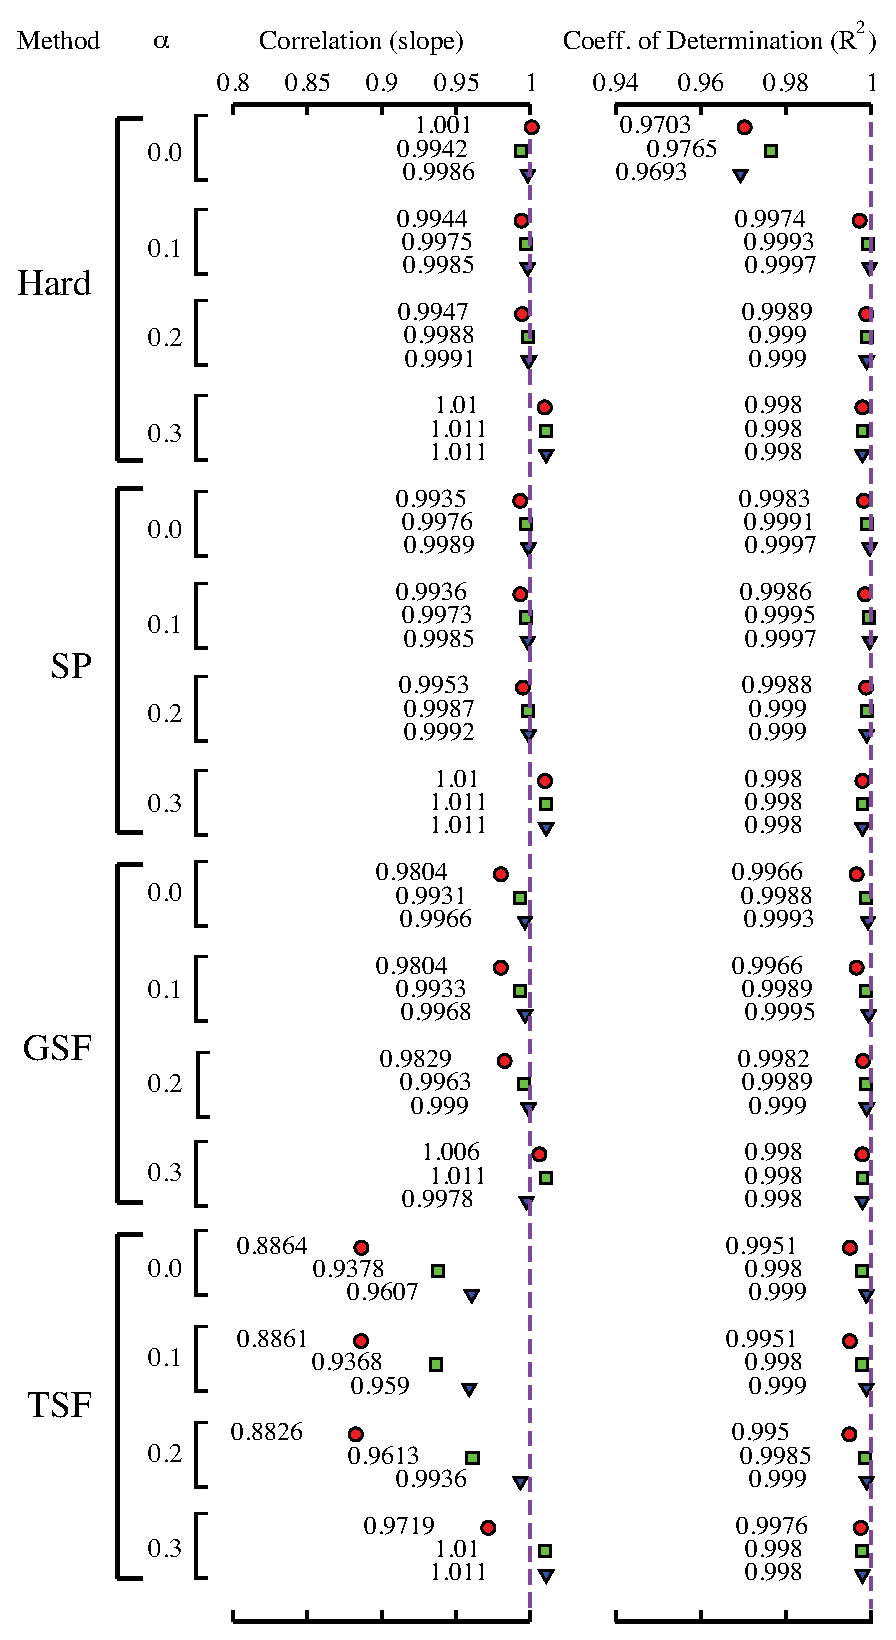
\includegraphics[width=0.6\linewidth]{energyPlot_slopeCorrelation_combined.eps}
  \caption{Statistical analysis of the quality of configurational
    energy differences for the real-space electrostatic methods
    compared with the reference Ewald sum.  Results with a value equal
    to 1 (dashed line) indicate $\Delta E$ values indistinguishable
    from those obtained using the multipolar Ewald sum.  Different
    values of the cutoff radius are indicated with different symbols
    (9~\AA\ = circles, 12~\AA\ = squares, and 15~\AA\ = inverted
    triangles).\label{fig:slopeCorr_energy}}
\end{figure} 

The combined coefficient of determination and slope for all six
systems is shown in Fig.~\ref{fig:slopeCorr_energy}.  Most of the
methods reproduce the Ewald configurational energy differences with
remarkable fidelity.  Undamped hard cutoffs introduce a significant
amount of random scatter in the energy differences which is apparent
in the reduced value of $R^2$ for this method.  This can be easily
understood as configurations which exhibit small traversals of a few
dipoles or quadrupoles out of the cutoff sphere will see large energy
jumps when hard cutoffs are used.  The orientations of the multipoles
(particularly in the ordered crystals) mean that these energy jumps
can go in either direction, producing a significant amount of random
scatter, but no systematic error.

The TSF method produces energy differences that are highly correlated
with the Ewald results, but it also introduces a significant
systematic bias in the values of the energies, particularly for
smaller cutoff values. The TSF method alters the distance dependence
of different orientational contributions to the energy in a
non-uniform way, so the size of the cutoff sphere can have a large
effect, particularly for the crystalline systems.

Both the SP and GSF methods appear to reproduce the Ewald results with
excellent fidelity, particularly for moderate damping ($\alpha \approx
0.2$~\AA$^{-1}$) and with a commonly-used cutoff value ($r_c =
12$~\AA).  With the exception of the undamped hard cutoff, and the TSF
method with short cutoffs, all of the methods would be appropriate for
use in Monte Carlo simulations.
\subsection{Magnitude of the force and torque vectors}

The comparisons of the magnitudes of the forces and torques for the
data accumulated from all six systems are shown in Fig.
~\ref{fig:slopeCorr_force} and \ref{fig:slopeCorr_torque}. The
correlation and slope for the forces agree well with the Ewald sum
even for the hard cutoffs.

For systems of molecules with only multipolar interactions, the pair
energy contributions are quite short ranged.  Moreover, the force
decays more rapidly than the electrostatic energy, hence the hard
cutoff method can also produce reasonable agreement for this quantity.
Although the pure cutoff gives reasonably good electrostatic forces
for pairs of molecules included within each other's cutoff spheres,
the discontinuity in the force at the cutoff radius can potentially
cause energy conservation problems as molecules enter and leave the
cutoff spheres.  This is discussed in detail in section
\ref{sec:conservation}.

The two shifted-force methods (GSF and TSF) exhibit a small amount of
systematic variation and scatter compared with the Ewald forces.  The
shifted-force models intentionally perturb the forces between pairs of
molecules inside each other's cutoff spheres in order to correct the
energy conservation issues, and this perturbation is evident in the
statistics accumulated for the molecular forces.  The GSF
perturbations are minimal, particularly for moderate damping and
commonly-used cutoff values ($r_c = 12$~\AA).  The TSF method shows
reasonable agreement in $R^2$, but again the systematic error in the
forces is concerning if replication of Ewald forces is desired.

It is important to note that the forces and torques from the SP and
the Hard cutoffs are not identical. The SP method shifts each
orientational contribution separately (e.g. the dipole-dipole dot
product is shifted by a different function than the dipole-distance
products), while the hard cutoff contains no orientation-dependent
shifting.  The forces and torques for these methods therefore diverge
for multipoles even though the forces for point charges are identical.

\begin{figure}
  \centering
  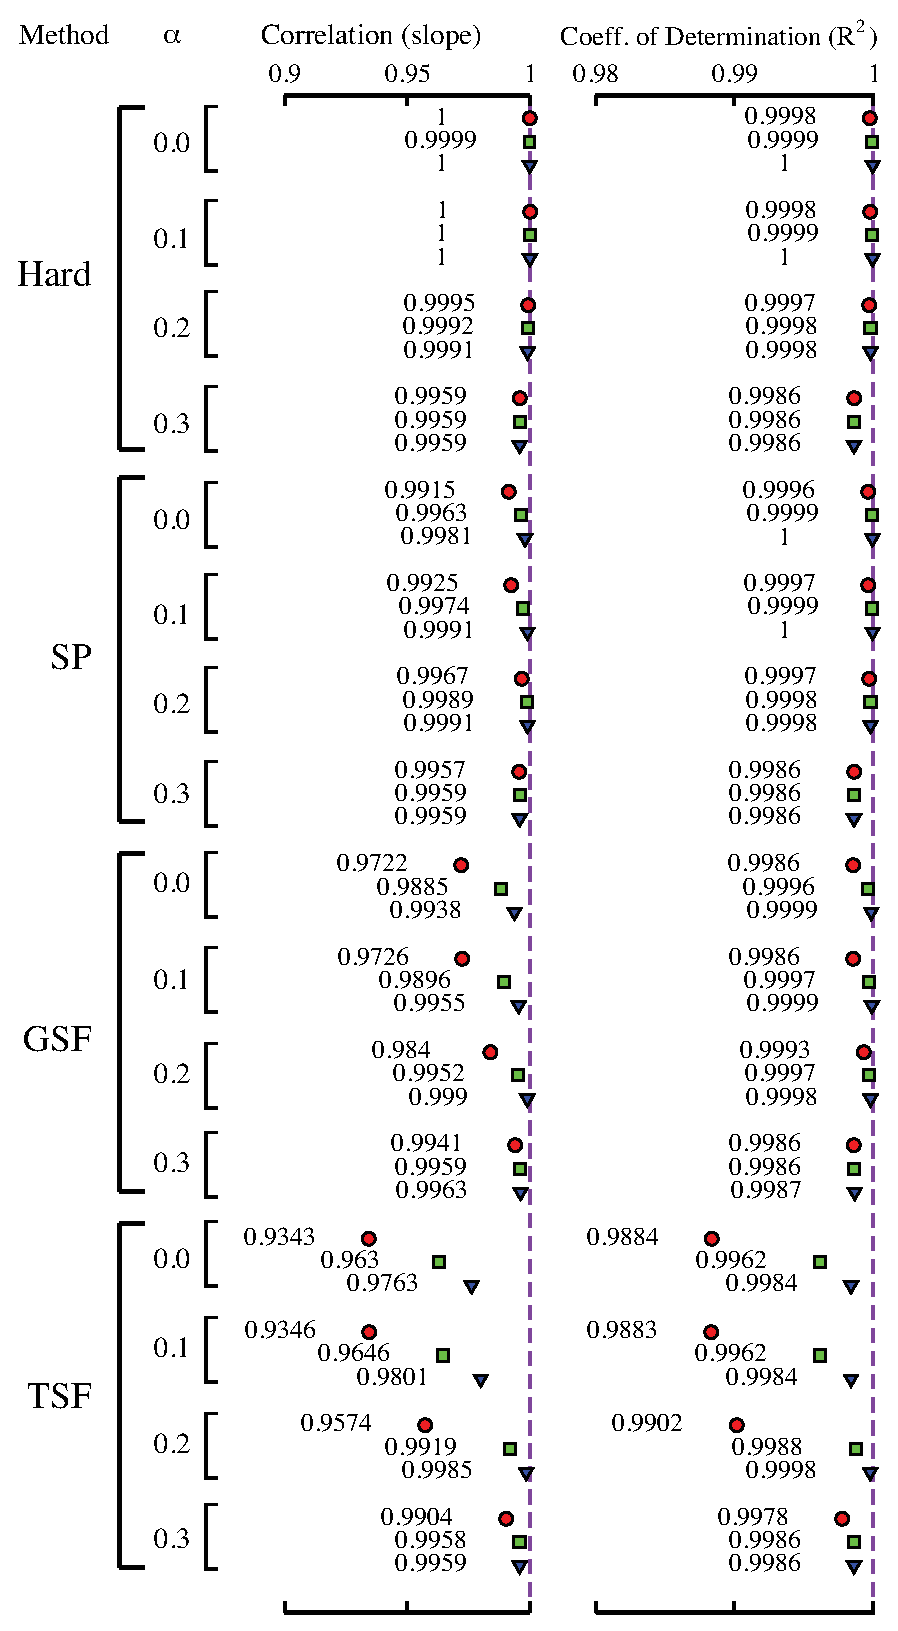
\includegraphics[width=0.6\linewidth]{forcePlot_slopeCorrelation_combined.eps} 
  \caption{Statistical analysis of the quality of the force vector
    magnitudes for the real-space electrostatic methods compared with
    the reference Ewald sum. Results with a value equal to 1 (dashed
    line) indicate force magnitude values indistinguishable from those
    obtained using the multipolar Ewald sum.  Different values of the
    cutoff radius are indicated with different symbols (9~\AA\ =
    circles, 12~\AA\ = squares, and 15~\AA\ = inverted
    triangles).\label{fig:slopeCorr_force}}
\end{figure} 


\begin{figure}
  \centering
  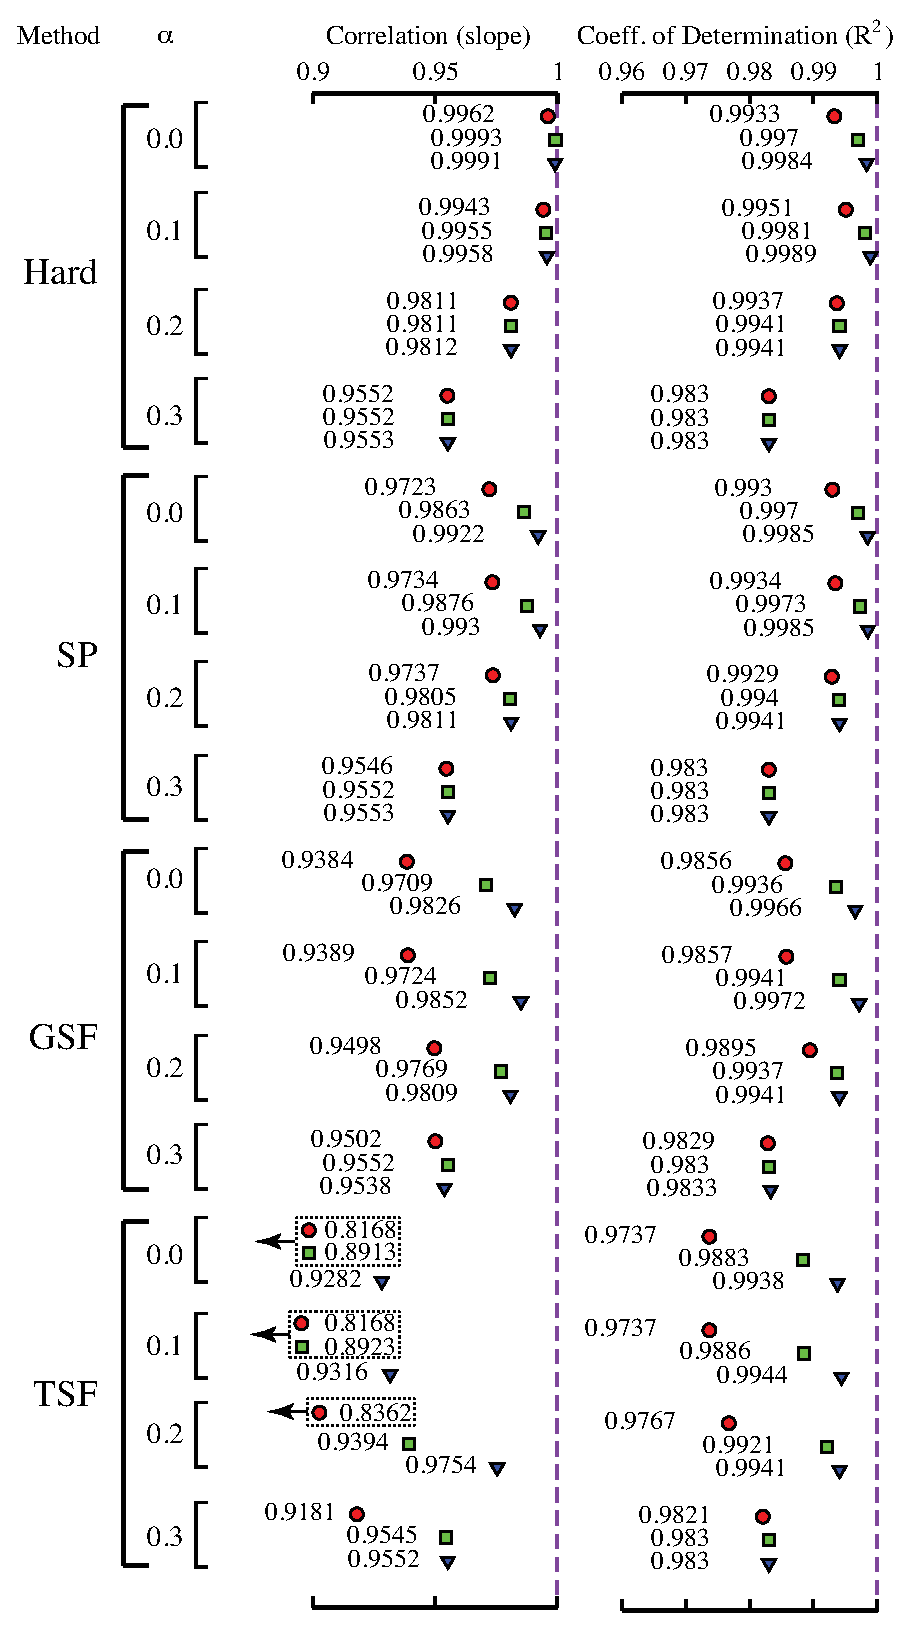
\includegraphics[width=0.6\linewidth]{torquePlot_slopeCorrelation_combined.eps}
  \caption{Statistical analysis of the quality of the torque vector
    magnitudes for the real-space electrostatic methods compared with
    the reference Ewald sum. Results with a value equal to 1 (dashed
    line) indicate force magnitude values indistinguishable from those
    obtained using the multipolar Ewald sum.  Different values of the
    cutoff radius are indicated with different symbols (9~\AA\ =
    circles, 12~\AA\ = squares, and 15~\AA\ = inverted
    triangles).\label{fig:slopeCorr_torque}}
\end{figure}

The torques (Fig. \ref{fig:slopeCorr_torque}) appear to be
significantly influenced by the choice of real-space method.  The
torque expressions have the same distance dependence as the energies,
which are naturally longer-ranged expressions than the inter-site
forces.  Torques are also quite sensitive to orientations of
neighboring molecules, even those that are near the cutoff distance.

The results shows that the torque from the hard cutoff method
reproduces the torques in quite good agreement with the Ewald sum.
The other real-space methods can cause some deviations, but excellent
agreement with the Ewald sum torques is recovered at moderate values
of the damping coefficient ($\alpha \approx 0.2$~\AA$^{-1}$) and cutoff
radius ($r_c \ge 12$~\AA).  The TSF method exhibits only fair agreement
in the slope when compared with the Ewald torques even for larger
cutoff radii.  It appears that the severity of the perturbations in
the TSF method are most in evidence for the torques.

\subsection{Directionality of the force and torque vectors}   

The accurate evaluation of force and torque directions is just as
important for molecular dynamics simulations as the magnitudes of
these quantities. Force and torque vectors for all six systems were
analyzed using Fisher statistics, and the quality of the vector
directionality is shown in terms of circular variance
($\mathrm{Var}(\theta)$) in
Fig. \ref{fig:slopeCorr_circularVariance}. The force and torque
vectors from the new real-space methods exhibit nearly-ideal Fisher
probability distributions (Eq.~\ref{eq:pdf}). Both the hard and SP
cutoff methods exhibit the best vectorial agreement with the Ewald
sum. The force and torque vectors from GSF method also show good
agreement with the Ewald method, which can also be systematically
improved by using moderate damping and a reasonable cutoff radius. For
$\alpha = 0.2$~\AA$^{-1}$ and $r_c = 12$~\AA, we observe
$\mathrm{Var}(\theta) = 0.00206$, which corresponds to a distribution
with 95\% of force vectors within $6.37^\circ$ of the corresponding
Ewald forces. The TSF method produces the poorest agreement with the
Ewald force directions.

Torques are again more perturbed than the forces by the new real-space
methods, but even here the variance is reasonably small.  For the same
method (GSF) with the same parameters ($\alpha = 0.2$~\AA$^{-1}$, $r_c
= 12$~\AA), the circular variance was 0.01415, corresponds to a
distribution which has 95\% of torque vectors are within $16.75^\circ$
of the Ewald results. Again, the direction of the force and torque
vectors can be systematically improved by varying $\alpha$ and $r_c$.

\begin{figure}
  \centering
  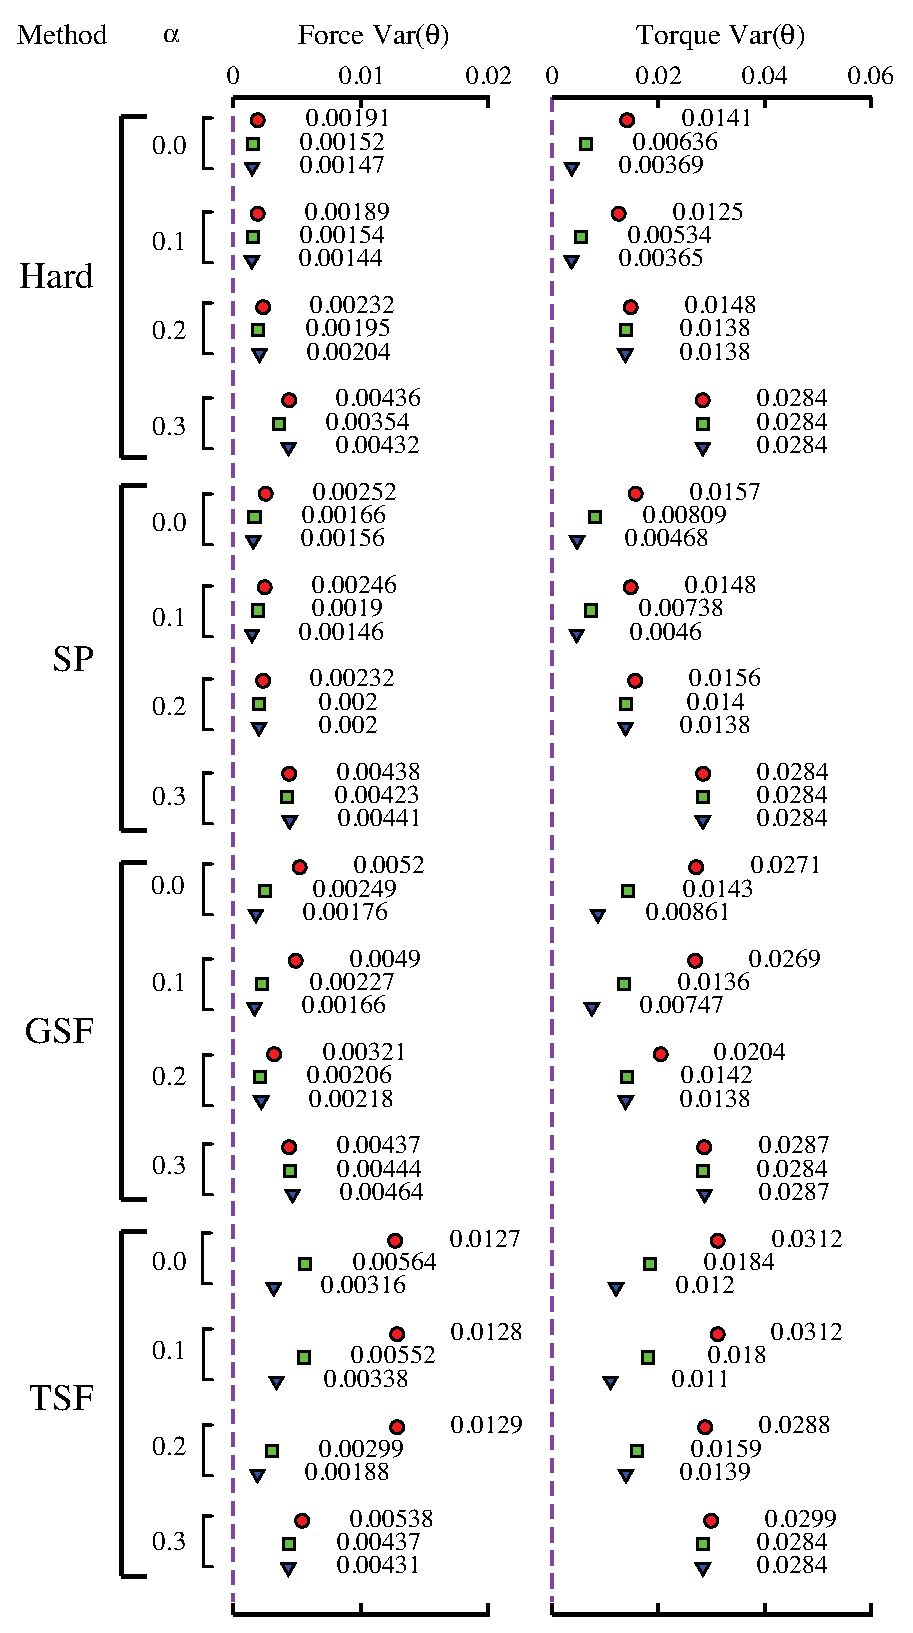
\includegraphics[width=0.65\linewidth]{Variance_forceNtorque_modified.eps}
  \caption{The circular variance of the direction of the force and
    torque vectors obtained from the real-space methods around the
    reference Ewald vectors. A variance equal to 0 (dashed line)
    indicates direction of the force or torque vectors are
    indistinguishable from those obtained from the Ewald sum. Here
    different symbols represent different values of the cutoff radius
    (9~\AA\ = circle, 12~\AA\ = square, 15~\AA\ = inverted triangle)\label{fig:slopeCorr_circularVariance}}
\end{figure}

\subsection{Energy conservation\label{sec:conservation}}

We have tested the conservation of energy one can expect to see with
the new real-space methods using the soft DQ liquid model with a small
fraction of solvated ions. This is a test system which exercises all
orders of multipole-multipole interactions derived in the chapter 2
in this series and provides the most comprehensive test of the new
methods.  A liquid-phase system was created with 2000 liquid-phase
molecules and 48 dissolved ions at a density of 0.98 g cm$^{-3}$ and a
temperature of 300K.  After equilibration in the canonical (NVT)
ensemble using a Nos\'e-Hoover thermostat, six
statistically-independent replicas of this liquid-phase system were
run in the microcanonical (NVE) ensemble under the Ewald, Hard, SP,
GSF, and TSF methods with a cutoff radius of 12~\AA.  The value of the
damping coefficient was also varied from the undamped case ($\alpha =
0$) to a heavily damped case ($\alpha = 0.3$~\AA$^{-1}$) for all of
the real space methods.  A sample was also run using the multipolar
Ewald sum with the same real-space cutoff.

In Fig.~\ref{fig:energyDrift} we show the both the linear drift in
energy over time, $\delta E_1$, and the standard deviation of energy
fluctuations around this drift $\delta E_0$.  Both of the
shifted-force methods (GSF and TSF) provide excellent energy
conservation (drift less than $10^{-5}$ kcal / mol / ns / particle),
while the hard cutoff is essentially unusable for molecular dynamics.
SP provides some benefit over the hard cutoff because the energetic
jumps that happen as particles leave and enter the cutoff sphere are
somewhat reduced, but like the Wolf method for charges, the SP method
would not be as useful for molecular dynamics as either of the
shifted-force methods.

We note that for all tested values of the cutoff radius, the new
real-space methods can provide better energy conservation behavior
than the multipolar Ewald sum, even when relatively large $k$-space
cutoff values are utilized.

\begin{figure}
  \centering
  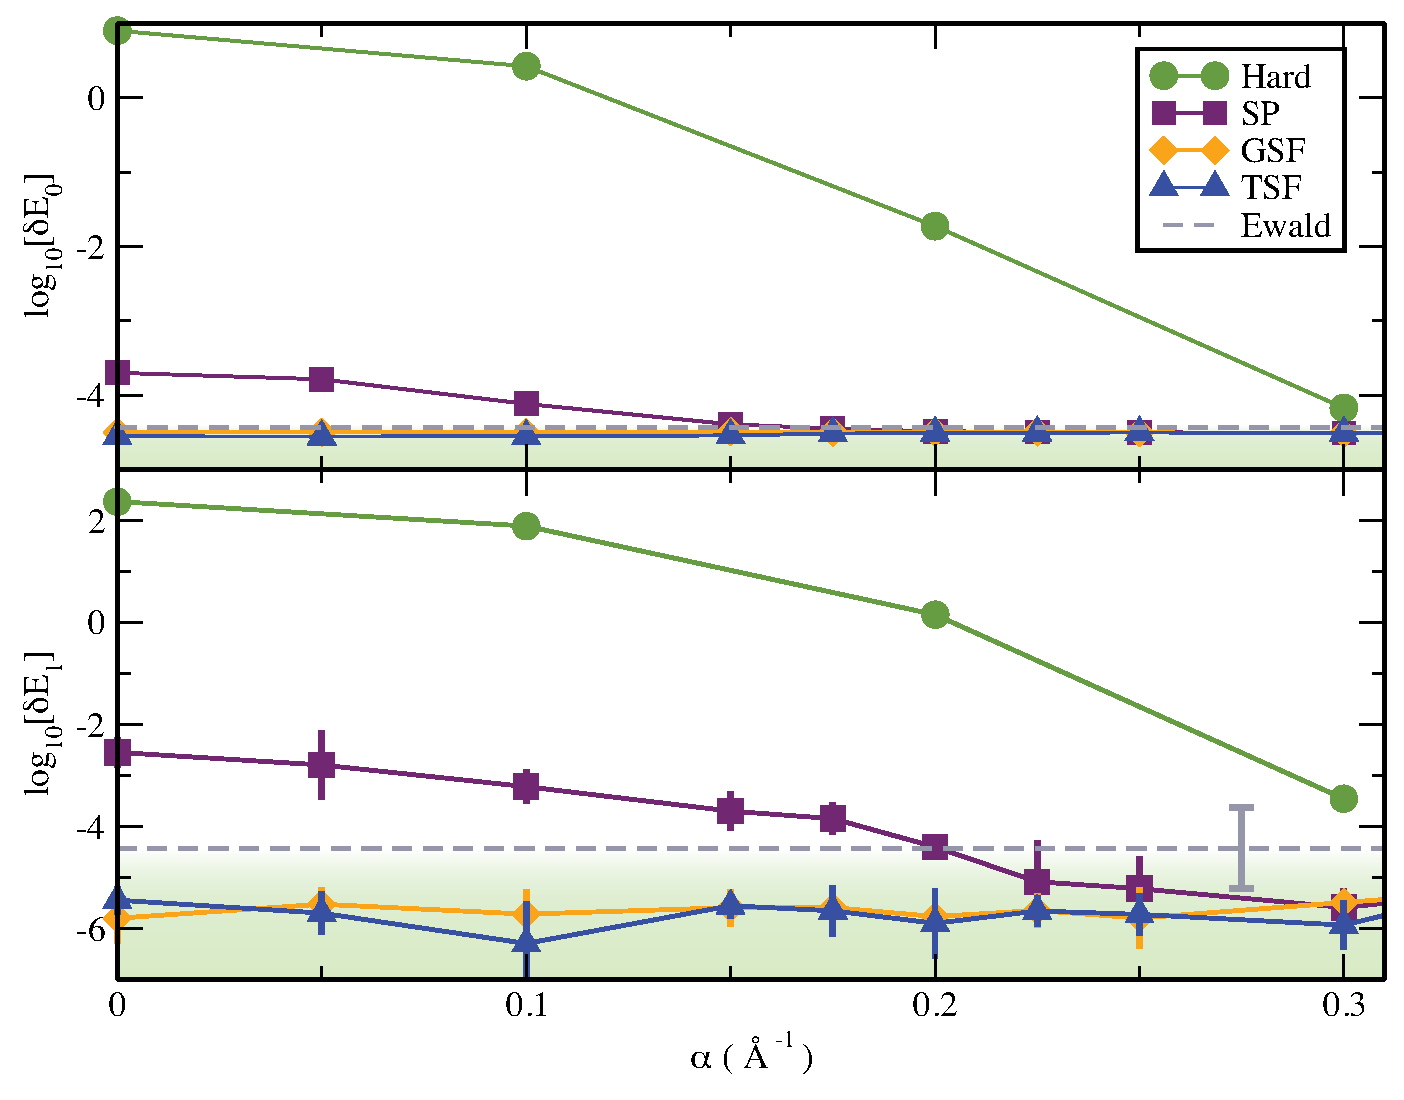
\includegraphics[width=\textwidth]{finalDrift.eps}
  \caption{Energy conservation of the real-space methods for the soft
    DQ liquid / ion system. $\delta \mathrm{E}_1$ is the linear drift
    in energy over time (in kcal/mol/particle/ns) and $\delta
    \mathrm{E}_0$ is the standard deviation of energy fluctuations
    around this drift (in kcal/mol/particle).  Points that appear in
    the green region at the bottom exhibit better energy conservation
    than would be obtained using common parameters for Ewald-based
    electrostatics.\label{fig:energyDrift}}
\end{figure} 
\subsection{Reproduction of Structural \& Dynamical Features\label{sec:structure}}
The most important test of the modified interaction potentials is the
fidelity with which they can reproduce structural features and
dynamical properties in a liquid.  One commonly-utilized measure of
structural ordering is the pair distribution function, $g(r)$, which
measures local density deviations in relation to the bulk density.  In
the electrostatic approaches studied here, the short-range repulsion
from the Lennard-Jones potential is identical for the various
electrostatic methods, and since short range repulsion determines much
of the local liquid ordering, one would not expect to see many
differences in $g(r)$.  Indeed, the pair distributions are essentially
identical for all of the electrostatic methods studied (for each of
the different systems under investigation). 

% An example of this agreement for the soft DQ liquid/ion system is
% shown in Fig. \ref{fig:gofr}.

% \begin{figure}
%   \centering
%   \includegraphics[width=\textwidth]{gofr_ssdqc.eps}
% \caption{The pair distribution functions, $g(r)$, for the SSDQ
%   water/ion system obtained using the different real-space methods are
%   essentially identical with the result from the Ewald
%   treatment.\label{fig:gofr}}
% \end{figure} 

There is a minor over-structuring of the first solvation shell when
using TSF or when overdamping with any of the real-space methods.
With moderate damping, GSF and SP produce pair distributions that are
identical (within numerical noise) to their Ewald counterparts.  The
degree of over-structuring can be measured most easily using the
coordination number,
\begin{equation}
n_C = 4\pi\rho \int_{0}^{a}r^2\text{g}(r)dr,
\end{equation}
where $\rho$ is the number density of the site-site pair interactions,
and $a$ is the radial location of the minima following the first peak
in $g(r)$ ($a = 4.2$~\AA\  for the soft DQ liquid / ion system).  The
coordination number is shown as a function of the damping coefficient
for all of the real space methods in Fig. \ref{fig:Props}.

A more demanding test of modified electrostatics is the average value
of the electrostatic energy $\langle U_\mathrm{elect} \rangle / N$
which is obtained by sampling the liquid-state configurations
experienced by a liquid evolving entirely under the influence of each
of the methods.  In Fig. \ref{fig:Props} we demonstrate how $\langle
U_\mathrm{elect} \rangle / N$ varies with the damping parameter,
$\alpha$, for each of the methods. 

As in the crystals studied in the chapter 2, damping is important
for converging the mean electrostatic energy values, particularly for
the two shifted force methods (GSF and TSF).  A value of $\alpha
\approx 0.2$~\AA$^{-1}$ is sufficient to converge the SP and GSF
energies with a cutoff of 12 \AA, while shorter cutoffs require more
dramatic damping ($\alpha \approx 0.28$~\AA$^{-1}$ for $r_c = 9$~\AA).
Overdamping the real-space electrostatic methods occurs with $\alpha >
0.3$~\AA$^{-1}$, causing the estimate of the electrostatic energy to
drop below the Ewald results.

These ``optimal'' values of the damping coefficient for structural
features are similar to those observed for DSF electrostatics for
purely point-charge systems, and the range $\alpha= 0.175 \rightarrow
0.225$~\AA$^{-1}$ for $r_c = 12$~\AA\ appears to be an excellent
compromise for mixed charge/multipolar systems.

To test the fidelity of the electrostatic methods at reproducing
\textit{dynamics} in a multipolar liquid, it is also useful to look at
transport properties, particularly the diffusion constant,
\begin{equation}
D = \lim_{t \rightarrow \infty} \frac{1}{6 t} \langle \left|
  \mathbf{r}(t) -\mathbf{r}(0) \right|^2 \rangle
\label{eq:diff}
\end{equation}
which measures long-time behavior and is sensitive to the forces on
the multipoles. The self-diffusion constants (D) were calculated from
linear fits to the long-time portion of the mean square displacement,
$\langle r^{2}(t) \rangle$.\cite{Allen89} In Fig. \ref{fig:Props} we
demonstrate how the diffusion constant depends on the choice of
real-space methods and the damping coefficient.  Both the SP and GSF
methods can obtain excellent agreement with Ewald again using moderate
damping.

In addition to translational diffusion, orientational relaxation times
were calculated for comparisons with the Ewald simulations and with
experiments. These values were determined by calculating the
orientational time correlation function,
\begin{equation}
C_l^\gamma(t) = \left\langle P_l\left[\hat{\mathbf{A}}_\gamma(t)
                \cdot\hat{\mathbf{A}}_\gamma(0)\right]\right\rangle,
\label{eq:OrientCorr}
\end{equation}
from the same 350 ps microcanonical trajectories that were used for
translational diffusion.  Here, $P_l$ is the Legendre polynomial of
order $l$ and $\hat{\mathbf{A}}_\gamma$ is the unit vector for body
axis $\gamma$.  The reference frame used for our sample dipolar
systems has the $z$-axis running along the dipoles, and for the soft
DQ liquid model, the $y$-axis connects the two implied hydrogen-like
positions.  From the orientation autocorrelation functions, we can
obtain time constants for rotational relaxation either by fitting to a
multi-exponential model for the orientational relaxation, or by
integrating the correlation functions.

In a good model for water, the orientational decay times would be
comparable to water orientational relaxation times from nuclear
magnetic resonance (NMR). The relaxation constant obtained from
$C_2^y(t)$ is normally of experimental interest because it describes
the relaxation of the principle axis connecting the hydrogen
atoms. Thus, $C_2^y(t)$ can be compared to the intermolecular portion
of the dipole-dipole relaxation from a proton NMR signal and can
provide an estimate of the NMR relaxation time constant.\cite{Impey82}
In Fig. \ref{fig:Props} we compare the $\tau_2^y$ and $\tau_2^z$
values for the various real-space methods over a range of different
damping coefficients.  The rotational relaxation for the $z$ axis
primarily probes the torques on the dipoles, while the relaxation for
the $y$ axis is sensitive primarily to the quadrupolar torques.

\begin{figure}
  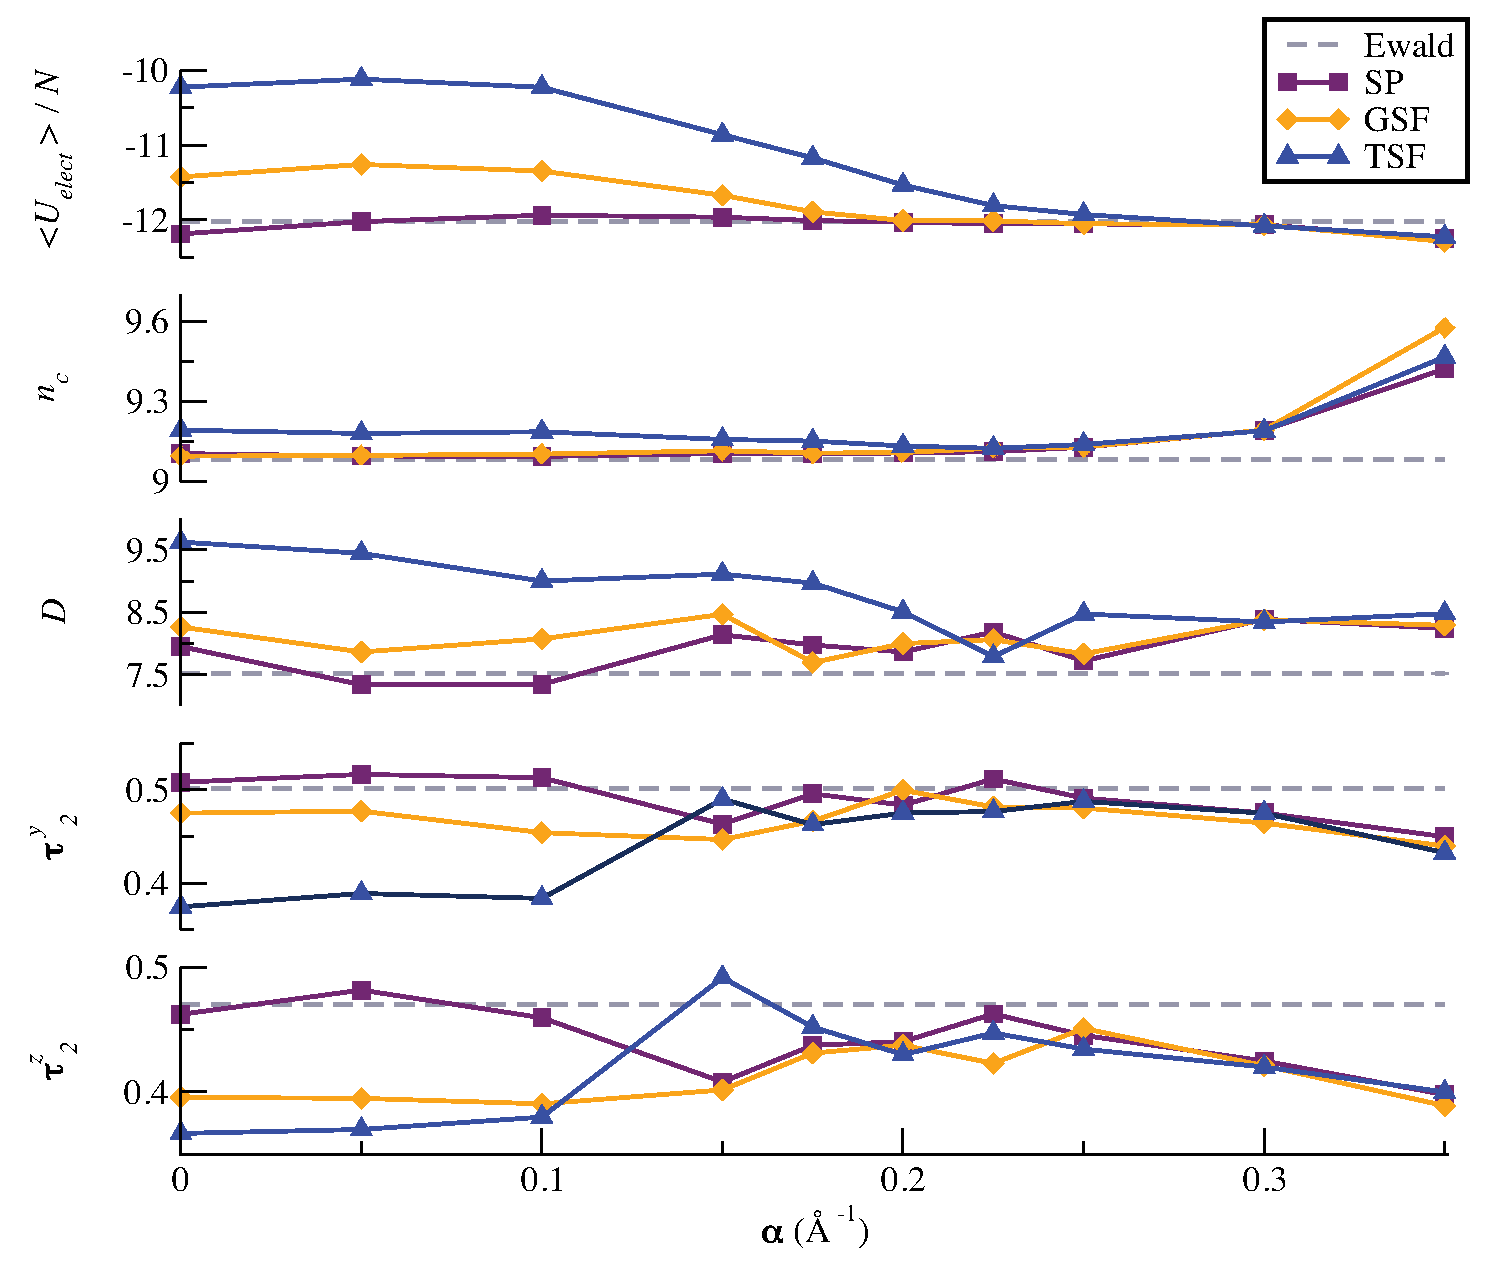
\includegraphics[width=\textwidth]{properties.eps}
  \caption{Comparison of the structural and dynamic properties for the
    combined multipolar liquid (soft DQ liquid + ions) for all of the
    real-space methods with $r_c = 12$~\AA. Electrostatic energies,
    $\langle U_\mathrm{elect} \rangle / N$ (in kcal / mol),
    coordination numbers, $n_C$, diffusion constants (in $10^{-5}
    \mathrm{cm}^2\mathrm{s}^{-1}$), and rotational correlation times
    (in ps) all show excellent agreement with Ewald results for
    damping coefficients in the range $\alpha= 0.175 \rightarrow
    0.225$~\AA$^{-1}$. \label{fig:Props}}
\end{figure}

In Fig. \ref{fig:Props} it appears that values for $D$, $\tau_2^y$,
and $\tau_2^z$ using the Ewald sum are reproduced with excellent
fidelity by the GSF and SP methods.  All of the real space methods can
be \textit{overdamped}, which reduces the effective range of multipole
interactions, causing structural and dynamical changes from the
correct behavior.  Because overdamping weakens orientational
preferences between adjacent molecules, it manifests as too-rapid
orientational decay coupled with faster diffusion and
over-coordination of the liquid.  Underdamping is less problematic for
the SP and GSF methods, as their structural and dynamical properties
still reproduce the Ewald results even in the completely undamped
($\alpha = 0$) case.  An optimal range for the electrostatic damping
parameter appears to be $\alpha= 0.175 \rightarrow 0.225$~\AA$^{-1}$
for $r_c = 12$~\AA, which similar to the optimal range found for the
damped shifted force potential for point charges.\cite{Gezelter06}

\section{Summary}
In the chapter 2, we generalized the
charge-neutralized electrostatic energy originally developed by Wolf
\textit{et al.}\cite{Wolf99} to multipole-multipole interactions
up to quadrupolar order.  The SP method is essentially a
multipole-capable version of the Wolf model.  The SP method for
multipoles provides excellent agreement with Ewald-derived energies,
forces and torques, and is suitable for Monte Carlo simulations,
although the forces and torques retain discontinuities at the cutoff
distance that prevents its use in molecular dynamics.

We also developed two natural extensions of the damped shifted-force
(DSF) model originally proposed by Zahn {\it et al.} and extended by
Fennell and Gezelter.\cite{Zahn02, Gezelter06} The GSF and TSF
approaches provide smooth truncation of energies, forces, and torques
at the real-space cutoff, and both converge to DSF electrostatics for
point-charge interactions.  The TSF model is based on a high-order
truncated Taylor expansion which can be relatively perturbative inside
the cutoff sphere.  The GSF model takes the gradient from an images of
the interacting multipole that has been projected onto the cutoff
sphere to derive shifted force and torque expressions, and is a
significantly more gentle approach.

The GSF method produces quantitative agreement with Ewald energies,
forces, and torques.  It also performs well in conserving energy in MD
simulations.  The Taylor-shifted (TSF) model provides smooth dynamics,
but these take place on a potential energy surface that is
significantly perturbed from Ewald-based electrostatics.  Because it
performs relatively poorly compared with GSF, it may seem odd that
that the TSF model was included in this work.  However, the functional
forms derived for the SP and GSF methods depend on the separation of
orientational contributions that were made visible by the Taylor
series of the electrostatic kernel at the cutoff radius. The TSF
method also has the unique property that a large number of derivatives
can be made to vanish at the cutoff radius.  This property has proven
useful in past treatments of the corrections to the Clausius-Mossotti
fluctuation formula for dielectric constants.\cite{Izvekov08}

Reproduction of both structural and dynamical features in the liquid
systems is remarkably good for both the SP and GSF models.  Pair
distribution functions are essentially equivalent to the same
functions produced using Ewald-based electrostatics, and with moderate
damping, a structural feature that directly probes the electrostatic
interaction (e.g. the mean electrostatic potential energy) can also be
made quantitative.  Dynamical features are sensitive probes of the
forces and torques produced by these methods, and even though the
smooth behavior of forces is produced by perturbing the overall
potential, the diffusion constants and orientational correlation times
are quite close to the Ewald-based results.

The only cases we have found where the new GSF and SP real-space
methods can be problematic are those which retain a bulk dipole moment
at large distances (e.g. the $Z_1$ dipolar lattice).  In ferroelectric
materials, uniform weighting of the orientational contributions can be
important for converging the total energy.  In these cases, the
damping function which causes the non-uniform weighting can be
replaced by the bare electrostatic kernel, and the energies return to
the expected converged values.

Based on the results of this work, we can conclude that the GSF method
is a suitable and efficient replacement for the Ewald sum for
evaluating electrostatic interactions in modern MD simulations, and
the SP method would be an excellent choice for Monte Carlo
simulations where smooth forces and energy conservation are not
important.  Both the SP and GSF methods retain excellent fidelity to
the Ewald energies, forces and torques.  Additionally, the energy
drift and fluctuations from the GSF electrostatics are significantly
better than a multipolar Ewald sum for finite-sized reciprocal spaces,
and physical properties are reproduced accurately.

As in all purely pairwise cutoff methods, the SP, GSF and TSF methods
are expected to scale approximately {\it linearly} with system size,
and are easily parallelizable.  This should result in substantial
reductions in the computational cost of performing large simulations.
With the proper use of pre-computation and spline interpolation of the
radial functions, the real-space methods are essentially the same cost
as a simple real-space cutoff.  They require no Fourier transforms or
$k$-space sums, and guarantee the smooth handling of energies, forces,
and torques as multipoles cross the real-space cutoff boundary.

We are not suggesting that there is any flaw with the Ewald sum; in
fact, it is the standard by which the SP, GSF, and TSF methods have
been judged in this work.  However, these results provide evidence
that in the typical simulations performed today, the Ewald summation
may no longer be required to obtain the level of accuracy most
researchers have come to expect.



% % uncomment the following lines,
% if using chapter-wise bibliography
%
% \bibliographystyle{ndnatbib}
% \bibliography{example}
